\documentclass[journal,12pt,twocolumn]{IEEEtran}

\usepackage{setspace}
\usepackage{gensymb}
\singlespacing
\usepackage[cmex10]{amsmath}

\usepackage{amsthm}

\usepackage{mathrsfs}
\usepackage{txfonts}
\usepackage{stfloats}
\usepackage{bm}
\usepackage{cite}
\usepackage{cases}
\usepackage{subfig}
\usepackage{tikz}
\usepackage{longtable}
\usepackage{multirow}

\usepackage{enumitem}
\usepackage{mathtools}
\usepackage{steinmetz}
\usepackage{tikz}
\usepackage{circuitikz}
\usepackage{verbatim}
\usepackage{tfrupee}
\usepackage[breaklinks=true]{hyperref}
\usepackage{graphicx}
\usepackage{tkz-euclide}

\usetikzlibrary{calc,math}
\usepackage{listings}
    \usepackage{color}                                            %%
    \usepackage{array}                                            %%
    \usepackage{longtable}                                        %%
    \usepackage{calc}                                             %%
    \usepackage{multirow}                                         %%
    \usepackage{hhline}                                           %%
    \usepackage{ifthen}                                           %%
    \usepackage{lscape}     
\usepackage{multicol}
\usepackage{chngcntr}

\DeclareMathOperator*{\Res}{Res}

\renewcommand\thesection{\arabic{section}}
\renewcommand\thesubsection{\thesection.\arabic{subsection}}
\renewcommand\thesubsubsection{\thesubsection.\arabic{subsubsection}}

\renewcommand\thesectiondis{\arabic{section}}
\renewcommand\thesubsectiondis{\thesectiondis.\arabic{subsection}}
\renewcommand\thesubsubsectiondis{\thesubsectiondis.\arabic{subsubsection}}


\hyphenation{op-tical net-works semi-conduc-tor}
\def\inputGnumericTable{}                                 %%

\lstset{
%language=C,
frame=single, 
breaklines=true,
columns=fullflexible
}
\begin{document}


\newtheorem{theorem}{Theorem}[section]
\newtheorem{problem}{Problem}
\newtheorem{proposition}{Proposition}[section]
\newtheorem{lemma}{Lemma}[section]
\newtheorem{corollary}[theorem]{Corollary}
\newtheorem{example}{Example}[section]
\newtheorem{definition}[problem]{Definition}

\newcommand{\BEQA}{\begin{eqnarray}}
\newcommand{\EEQA}{\end{eqnarray}}
\newcommand{\define}{\stackrel{\triangle}{=}}
\bibliographystyle{IEEEtran}
\raggedbottom
\setlength{\parindent}{0pt}
\providecommand{\mbf}{\mathbf}
\providecommand{\pr}[1]{\ensuremath{\Pr\left(#1\right)}}
\providecommand{\qfunc}[1]{\ensuremath{Q\left(#1\right)}}
\providecommand{\sbrak}[1]{\ensuremath{{}\left[#1\right]}}
\providecommand{\lsbrak}[1]{\ensuremath{{}\left[#1\right.}}
\providecommand{\rsbrak}[1]{\ensuremath{{}\left.#1\right]}}
\providecommand{\brak}[1]{\ensuremath{\left(#1\right)}}
\providecommand{\lbrak}[1]{\ensuremath{\left(#1\right.}}
\providecommand{\rbrak}[1]{\ensuremath{\left.#1\right)}}
\providecommand{\cbrak}[1]{\ensuremath{\left\{#1\right\}}}
\providecommand{\lcbrak}[1]{\ensuremath{\left\{#1\right.}}
\providecommand{\rcbrak}[1]{\ensuremath{\left.#1\right\}}}
\theoremstyle{remark}
\newtheorem{rem}{Remark}
\newcommand{\sgn}{\mathop{\mathrm{sgn}}}
% \providecommand{\abs}[1]{\left\vert#1\right\vert}
% \providecommand{\res}[1]{\Res\displaylimits_{#1}} 
% \providecommand{\norm}[1]{\left\lVert#1\right\rVert}
% %\providecommand{\norm}[1]{\lVert#1\rVert}
% \providecommand{\mtx}[1]{\mathbf{#1}}
% \providecommand{\mean}[1]{E\left[ #1 \right]}
\providecommand{\fourier}{\overset{\mathcal{F}}{ \rightleftharpoons}}
%\providecommand{\hilbert}{\overset{\mathcal{H}}{ \rightleftharpoons}}
\providecommand{\system}{\overset{\mathcal{H}}{ \longleftrightarrow}}
	%\newcommand{\solution}[2]{\textbf{Solution:}{#1}}
\newcommand{\solution}{\noindent \textbf{Solution: }}
\newcommand{\cosec}{\,\text{cosec}\,}
\providecommand{\dec}[2]{\ensuremath{\overset{#1}{\underset{#2}{\gtrless}}}}
\newcommand{\myvec}[1]{\ensuremath{\begin{pmatrix}#1\end{pmatrix}}}
\newcommand{\mydet}[1]{\ensuremath{\begin{vmatrix}#1\end{vmatrix}}}
\numberwithin{equation}{subsection}
\def\putbox#1#2#3{\makebox[0in][l]{\makebox[#1][l]{}\raisebox{\baselineskip}[0in][0in]{\raisebox{#2}[0in][0in]{#3}}}}
     \def\rightbox#1{\makebox[0in][r]{#1}}
     \def\centbox#1{\makebox[0in]{#1}}
     \def\topbox#1{\raisebox{-\baselineskip}[0in][0in]{#1}}
     \def\midbox#1{\raisebox{-0.5\baselineskip}[0in][0in]{#1}}
\vspace{3cm}
\title{Assignment 1}
\author{Aayush Goyal - EE18BTECH11001}
\maketitle
\newpage
\bigskip
Github repository
%
\begin{lstlisting}
https://github.com/aayush2710/EE4013-Assignment1
\end{lstlisting}
\setcounter{figure}{0}
\section{Problem}
Consider the following Recurrence Relation
\begin{multline}
  T\brak{n} =
  \begin{cases}
  T\brak{n/2} + T\brak{2n/5} + 7n & \text{if } n>0 \\
  1 & \text{if } n=0
  \end{cases}
\end{multline}

Which one of the following options is correct?
\begin{enumerate}
    \item $T\brak{n} = \mathcal{O}\brak{n^{\frac{5}{2}}}$
    \item $T\brak{n} = \mathcal{O}\brak{n\log n}$
    \item $T\brak{n} = \mathcal{O}\brak{n}$
    \item $T\brak{n} = \mathcal{O}\brak{\brak{\log n}^{\frac{5}{2}}}$
\end{enumerate}
\section{Solution}
Let us start by drawing the recurrence tree for the given problem. We can calculate the complexity of each level by summing up the complexity of each node at that level.\\ For Example : At L1, complexity is \\
$7\brak{\dfrac{n}{2}} + 7\brak{\dfrac{2n}{5}} = 7\brak{\dfrac{9n}{10}}$
\\

\begin{figure}[!h]
\centering
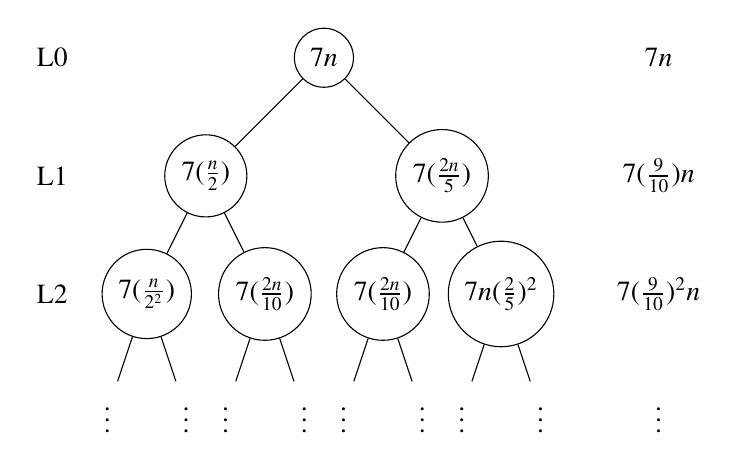
\begin{tikzpicture}[level/.style={sibling distance=30mm/#1}]
\node [circle,draw] (z){$7n$}
  child {node [circle,draw] (a) {$7(\frac{n}{2})$}
    child {node [circle,draw] (b) {$7(\frac{n}{2^2})$}
      child {node {$\vdots$}
      child [grow=left, xshift=0.8cm] {node (r) {} edge from parent[draw=none]
      child [grow=up] {node (s) {L2} edge from parent[draw=none]
      child [grow=up] {node (t) {L1} edge from parent[draw=none]
      child [grow=up] {node (t) {L0} edge from parent[draw=none]}}}}
      } 
      child {node {$\vdots$}}
    }
    child {node [circle,draw] (g) {$7(\frac{2n}{10})$}
      child {node {$\vdots$}}
      child {node {$\vdots$}}
    }
  }
  child {node [circle,draw] (j) {$7(\frac{2n}{5})$}
    child {node [circle,draw] (k) {$7(\frac{2n}{10})$}
      child {node {$\vdots$}}
      child {node {$\vdots$}}
    }
  child {node [circle,draw] (l) {$7n(\frac{2}{5})^2$}
    child {node {$\vdots$}}
    child {node (c){$\vdots$}
            child [grow=right] {node (r) {$\vdots$} edge from parent[draw=none]
              child [grow=up] {node (s) {$7(\frac{9}{10})^2 n$} edge from parent[draw=none]
                child [grow=up] {node (t) {$7(\frac{9}{10})n$} edge from parent[draw=none]
                  child [grow=up] {node (u) {$7n$} edge from parent[draw=none]}
                }
              }
            }
    }
  }
};

\end{tikzpicture}
\caption{Recurrence Tree} \label{fig:M1}
\end{figure}

Length of left most subtree $=\log_{2}n$\\
Length of right most subtree $=\log_{5/2}n$\\
Rightmost subtree is shortest so it determines the lower bound of time. Whereas the leftmost subtree is the longest, hence it determies the upper bound of time.


Height of the leftmost subtree is : $\log_{2}n $ and so

\begin{align}
T\brak{n} &\leqslant 7n + 7n\brak{\frac{9}{10}} + 7n\brak{\frac{9}{10}}^2  + \dots + 7n\brak{\frac{9}{10}}^{\log_{2}n} \\
T\brak{n} &\leqslant 7n\brak{1 + \frac{9}{10} + 7\brak{\frac{9}{10}}^2 + \dots + 7\brak{\frac{9}{10}}^{\log_{2}n}} \\
T\brak{n} &\leqslant 7n\dfrac{1-\brak{\dfrac{9}{10}}^{\log_{2} n + 1}}{1-\dfrac{9}{10}} \\
T\brak{n} &\leqslant 70n - 70\brak{\frac{9}{10}}\brak{n^{\log_{2}\brak{\frac{9}{10}}} } \\
&= 70n - 63n^{0.85}
\end{align}
\begin{flalign}
&\implies T\brak{n} \leqslant 70n & \\
&\implies T\brak{n} \in \mathcal{O}\brak{n}&
\end{flalign}

Height of the rightmost subtree is $log_{_{5/2}}n$ and so,

\begin{align}
T\brak{n} &\geqslant 7n + 7n\brak{\frac{9}{10}} + 7n\brak{\frac{9}{10}}^2 + \dots + 7n\brak{\frac{9}{10}}^{\log_{5/2}n}\\
T\brak{n} &\geqslant 7n\brak{1 + \frac{9}{10} + 7\brak{\frac{9}{10}}^2 + \dots + 7\brak{\frac{9}{10}}^{\log_{5/2}n}} \\
T\brak{n} &\geqslant 7n\dfrac{1-\brak{\dfrac{9}{10}}^{\brak{\log_{5/2}n} + 1}}{1-\dfrac{9}{10}}
\end{align}
\begin{align}
T\brak{n} &\geqslant 70n - 70\brak{\frac{9}{10}}\brak{n^{\log_{5/2} \brak{\frac{9}{10}}}} \\
&= 70n - 63n^{0.89} \\
T\brak{n} &\geqslant n\brak{70 - \frac{63}{n^{0.11}}}
\end{align}

Since we consider complexity for large n,
$\lim_{n \to \infty} \dfrac{63}{n^{0.11}} = 0$
So $T\brak{n} \geqslant 70n$

\section{Answer}
\begin{flalign}
&\bullet T\brak{n} \in \mathcal{O}\brak{n}& \\
&\bullet T\brak{n} \sim 70n &
\end{flalign}
Hence option 3 is correct

\section{Verification}
To verify the theoretical results, I constructed a recursive function in C with given recurrence relation and measure the execution time for different n.

The time taken was plotted using python with varying n, Here is the plot

\begin{figure}[!h]
    \centering
    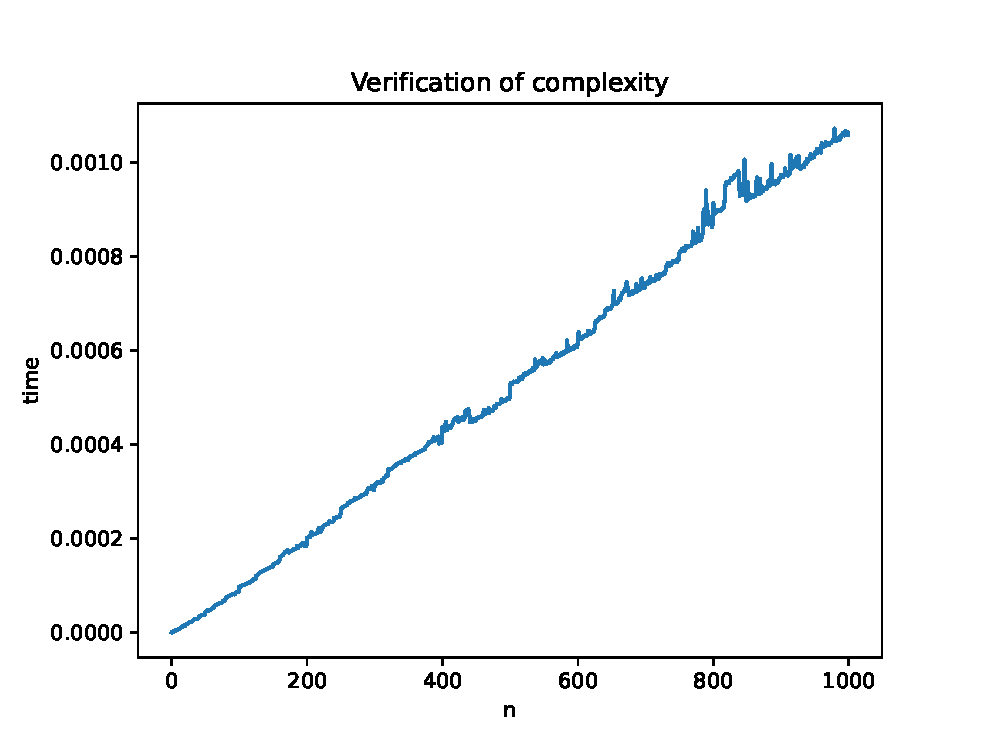
\includegraphics[scale=0.55]{figs/plot.eps}
    \caption{T\brak{n} vs n}
    \label{fig:verification}
\end{figure}
\\
We can clearly observe a linear curve. This verifies that 
$T\brak{n} \in \mathcal{O}\brak{n}$
\\
\\
Using least squares, approximate time equation is 

$T(n) = 0.091944n -1.917707$
\\
\\
Here is the recursive function used
\\
\begin{lstlisting}
void recursive(int n) {
    if(n == 0) {
      return;
    }
    long long int Sum = 0;
    for(int i=0;i<7*n;i++){ 
        Sum+=i;
    }
    recursive(n/2);
    recursive(2*n/5);
}
\end{lstlisting}
\\
\\
This plot can be generated through the following python script
\begin{lstlisting}
https://github.com/aayush2710/EE4013-Assignment1/code/verification.py
\end{lstlisting}
\end{document}

